\documentclass[tikz,border=8pt]{standalone}
\usepackage{tikz}
\usetikzlibrary{positioning,calc,arrows.meta}

\begin{document}
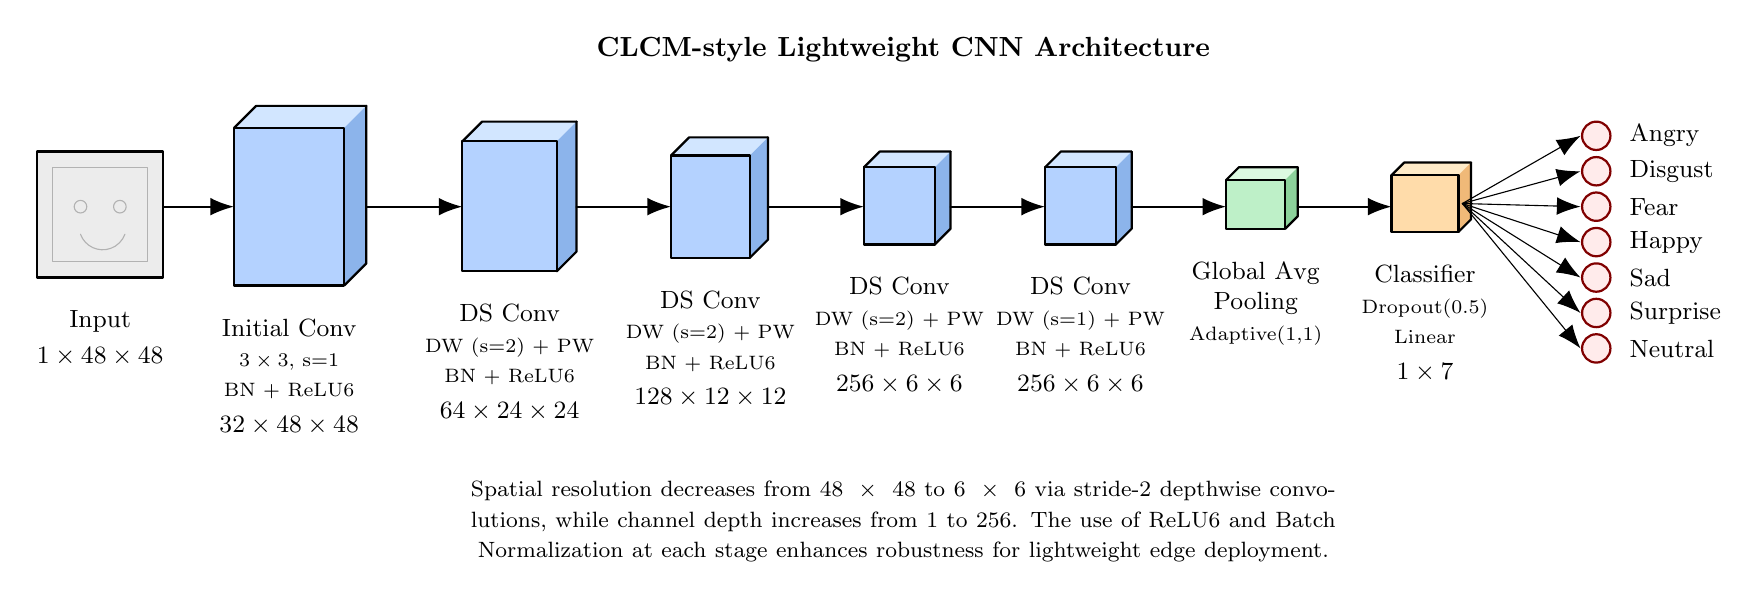
\begin{tikzpicture}[
    font=\small,
    >={Latex[length=3mm]},
    line join=round,
    line cap=round
]

% ========= Colors =========
\definecolor{convcolor}{RGB}{180,210,255}
\definecolor{convtop}{RGB}{210,230,255}
\definecolor{convside}{RGB}{140,180,235}

\definecolor{poolcolor}{RGB}{190,240,200}
\definecolor{pooltop}{RGB}{220,250,225}
\definecolor{poolside}{RGB}{140,210,155}

\definecolor{fccolor}{RGB}{255,220,170}
\definecolor{fctop}{RGB}{255,235,200}
\definecolor{fcside}{RGB}{240,185,120}

\definecolor{outcolor}{RGB}{255,235,235}

% ========= Helper: pseudo-3D block =========
% args: x, y, w, h, d, front, top, side, label
\newcommand{\cubeblock}[9]{
    % front
    \fill[#6] (#1,#2) rectangle ++(#3,#4);
    % top
    \fill[#7] (#1,#2+#4) -- ++(#5,#5) -- ++(#3,0) -- ++(-#5,-#5) -- cycle;
    % side
    \fill[#8] (#1+#3,#2) -- ++(#5,#5) -- ++(0,#4) -- ++(-#5,-#5) -- cycle;

    % outlines
    \draw[thick] (#1,#2) rectangle ++(#3,#4);
    \draw[thick] (#1,#2+#4) -- ++(#5,#5) -- ++(#3,0);
    \draw[thick] (#1+#3,#2) -- ++(#5,#5) -- ++(0,#4);

    % label (Anchor set to north to prevent upward overlapping)
    \node[align=center, anchor=north] at ($(#1,#2)+(#3/2,-0.3)$) {#9};
}

% ========= Input image =========
\draw[fill=gray!15, thick] (0,0.1) rectangle (1.6,1.7);
\draw[gray!60] (0.2,0.3) rectangle (1.4,1.5);
\draw[gray!60] (0.55,1.0) circle (0.08);
\draw[gray!60] (1.05,1.0) circle (0.08);
\draw[gray!60] (0.55,0.65) arc[start angle=200,end angle=340,radius=0.3];
\node[align=center, anchor=north] at (0.8,-0.2) {Input\\[0.5ex]$1\times48\times48$};

% ========= Blocks (X-coordinates expanded for text clearance) =========
\cubeblock{2.5}{0.0}{1.4}{2.0}{0.28}{convcolor}{convtop}{convside}{Initial Conv\\ \scriptsize $3\times3$, s=1\\ \scriptsize BN + ReLU6\\[0.5ex] $32\times48\times48$}

\cubeblock{5.4}{0.18}{1.2}{1.65}{0.25}{convcolor}{convtop}{convside}{DS Conv\\ \scriptsize DW (s=2) + PW\\ \scriptsize BN + ReLU6\\[0.5ex] $64\times24\times24$}

\cubeblock{8.05}{0.35}{1.0}{1.30}{0.23}{convcolor}{convtop}{convside}{DS Conv\\ \scriptsize DW (s=2) + PW\\ \scriptsize BN + ReLU6\\[0.5ex] $128\times12\times12$}

\cubeblock{10.5}{0.52}{0.9}{0.98}{0.20}{convcolor}{convtop}{convside}{DS Conv\\ \scriptsize DW (s=2) + PW\\ \scriptsize BN + ReLU6\\[0.5ex] $256\times6\times6$}

\cubeblock{12.8}{0.52}{0.9}{0.98}{0.20}{convcolor}{convtop}{convside}{DS Conv\\ \scriptsize DW (s=1) + PW\\ \scriptsize BN + ReLU6\\[0.5ex] $256\times6\times6$}

\cubeblock{15.1}{0.72}{0.75}{0.62}{0.16}{poolcolor}{pooltop}{poolside}{Global Avg\\Pooling\\ \scriptsize Adaptive(1,1)}

\cubeblock{17.2}{0.68}{0.85}{0.72}{0.16}{fccolor}{fctop}{fcside}{Classifier\\ \scriptsize Dropout(0.5)\\ \scriptsize Linear\\[0.5ex] $1\times7$}

% ========= Output nodes =========
\foreach \y/\lab in {1.9/Angry,1.45/Disgust,1.0/Fear,0.55/Happy,0.10/Sad,-0.35/Surprise,-0.80/Neutral}
{
    \filldraw[fill=outcolor,draw=red!50!black,thick] (19.8,\y) circle (0.18);
    \node[right] at (20.1,\y) {\lab};
}

% ========= Arrows (Recalculated for new spacing) =========
\draw[->,thick] (1.6,1.0) -- (2.5,1.0);
\draw[->,thick] (4.18,1.0) -- (5.4,1.0);
\draw[->,thick] (6.85,1.0) -- (8.05,1.0);
\draw[->,thick] (9.28,1.0) -- (10.5,1.0);
\draw[->,thick] (11.6,1.0) -- (12.8,1.0);
\draw[->,thick] (13.9,1.0) -- (15.1,1.0);
\draw[->,thick] (16.01,1.0) -- (17.2,1.0);

\foreach \y in {1.9,1.45,1.0,0.55,0.10,-0.35,-0.80}
{
    \draw[->,thin] (18.1,1.04) -- (19.6,\y);
}

% ========= Optional title =========
\node[font=\bfseries] at (11.0,3.0) {CLCM-style Lightweight CNN Architecture};

% ========= Optional note (Moved further down to avoid overlap) =========
\node[align=center, text width=16cm] at (11.0,-3.0)
{\footnotesize
Spatial resolution decreases from $48\times48$ to $6\times6$ via stride-2 depthwise convolutions, while channel depth increases from 1 to 256. The use of ReLU6 and Batch Normalization at each stage enhances robustness for lightweight edge deployment.};

\end{tikzpicture}
\end{document}
